\documentclass[10pt, a4paper, twocolumn]{article}
\usepackage{bachelorproject}
\title{\vspace{-0.5in}
	\textbf{\textsc{Biologically plausible model of human learning in simple arithmetic tasks}}\\\vspace{1ex}
	\normalsize{Bachelor's Project Thesis}\vspace{-2ex}}
\author{
	\normalsize{Boris Radovanovic, s3301419, b.radovanovic@student.rug.nl}\\ 
	\normalsize{Supervisor: Dr Jelmer P. Borst}}
\date{\vspace{-5ex}}

\begin{document}
	
\twocolumn[
\maketitle
\begin{abstract}
How we learn to perform simple arithmetic tasks is not thoroughly understood. Generally it is known that we first follow a procedure to reach a solution, and that we memorize previous solutions over time, however, it is not yet known how the transition between these strategies happens on a neuronal level. Several cognitive models using spiking neural networks were developed in hopes of explaining this mechanism, however they were generally very brittle against changes to inputs or hyperparameters. In this paper we present a cognitive model capable of solving alphabet arithmetic problems implemented in spiking neurons. The model initially uses a counting strategy and switches to a recall strategy over time. The model is built around a clock circuit that synchronizes its actions, which made it significantly simpler to develop and reason about while also making it robust against changes in hyperparameters and generalizable across different inputs. The model shows similar patterns in response times as those from human experimental results. Hopefully, it can serve as a groundwork for a future model that can completely recreate the human timings.
\end{abstract}
\vspace{6ex}]
	
\thispagestyle{firststyle}
	
\section{Introduction}
	
\cite{Fitts1967} proposed that each person goes through distinct \emph{learning phases} when acquiring a new skill - such as when children learn how to add numbers. The first phase is the \emph{cognitive phase}, in which an algorithm or rule is followed to produce the answer. For example, in this phase, a child may add 3+3 simply by counting up from 3 to 6. After the same addition problem is repeated many times, the child will eventually memorize the answer and enter the so-called \emph{associative phase}. In this phase, the answer is directly retrieved from long-term memory without any computation. Thus, producing the answer in the associative phase is much faster than in the cognitive phase.

\cite{Fitts1967} also proposed a third, \emph{autonomous phase}, which occurs when the answer has been repeated so many times that it becomes ingrained in procedural (muscle) memory. In this phase, answering a problem becomes almost instinctive.

Several experiments have supported the existence of these learning phases, and one of the most extensively modeled and studied experiments was done by \cite{Zbrodoff1995}. In Zbrodoff's experiment, participants learned to solve simple \emph{alphabet arithmetic} tasks such as verifying whether A+2=C. The results from the experiment are summarized in Table \ref{table:zbrodoff}. 

\begin{table}[h]
	\centering
	\begin{tabular}{cccc}
		block & X+2    & X+3    & X+4    \\\hline
		1     & 1\,728 & 2\,293 & 2\,727 \\
		2     & 1\,136 & 1\,345 & 1\,317 \\
		3     & 1\,077 & 1\,143 & 1\,131 \\
	\end{tabular}
	\caption{Human mean response times in milliseconds to alphabet arithmetic problems from Zbrodoff's experiment as a function of experiment block and addend. Summarized from \cite{Zbrodoff1995}.}
	\label{table:zbrodoff}
\end{table}

As can be seen from the table, response times generally decreased over time as the participants memorized their previous answers to the problems. Most notably, the difference in response times between the different addends was smaller in the later blocks. This is consistent with the idea that people first count, which takes more time for larger addends, and then later recall, which should take approximately the same amount of time regardless of the addend. Overall, this is consistent with a transition from the cognitive learning phase to the associative learning phase.

In order to better understand how the human cognitive system undergoes the transition between learning phases, several cognitive models such as the one by \cite{Lebiere1999} were developed in the \emph{ACT-R} cognitive modelling framework. More recently, the ACT-R tutorial unit on learning focuses on a model of the Zbrodoff task. The reference implementation of this model initially counts to reach the answer, and then switches to a recall strategy over time as answers are memorized. The results of this model match the experimental data very closely, as can be seen in Figure \ref{fig:actr-zbrodoff}.

\begin{figure}[h]
	\centering
	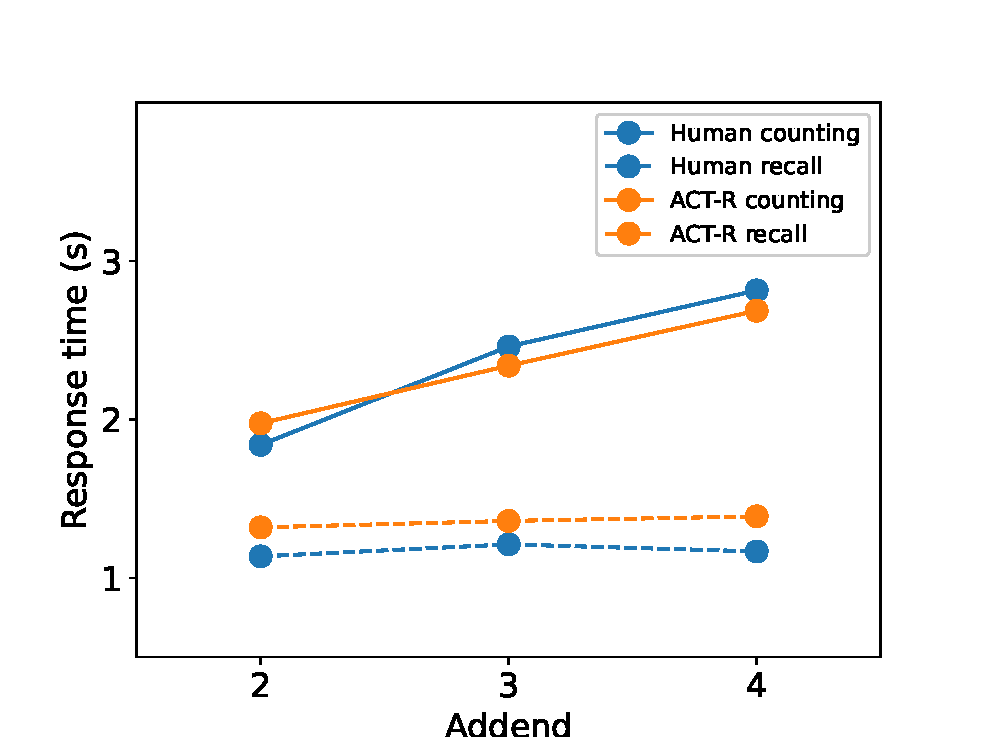
\includegraphics[width=1.0\linewidth]{figures/actr-zbrodoff.eps}
	\caption{A comparison of the response times of the ACT-R model and the experimental data in block 1 (counting) and block 3 (recall). Solid lines represent the counting strategy response times, while dashed lines represent the recall strategy response times.}
	\label{fig:actr-zbrodoff}
\end{figure}

ACT-R models the brain at the granularity of individual brain regions \citep{Anderson2004}. As such, ACT-R models of the Zbrodoff experiment generally match the experimental data closely and are good at predicting which brain regions are involved in the process of solving the task. However, they still do not explain how the transition between learning phases happens on a neuronal level.
	
\cite{Aubin2016} have successfully modeled the transition between the learning phases in spiking neural networks using Nengo, which is another cognitive modeling framework \citep{Nengo}. Their model performed addition, but it used 2 separate neural networks for retrieval and counting, which worked in parallel. This parallel process strategy, which was initially proposed by \cite{Logan1988} is not consistent with the theory of \cite{Fitts1967}. Additionally, the ACT-R model matched human response times without this parallel strategy, which indicates that a simpler, serial strategy would better model the brain.
	
Finally, \cite{Praetorius} designed a partially working Nengo model of the Zbrodoff task. The model was able to successfully count to the answer, memorize it, and then recall it in a later trial. However, due to the large amount of noise in the model, its behavior was very unstable, and this result was only observed once. \citeauthor{Praetorius} concluded by saying, ``It is in principle possible to create a Nengo model capable of recreating behavioral data from the Zbrodoff task".
	
In this project, we attempt to develop a neural model of learning which is capable of transitioning from the cognitive to the associative phase. Ideally, the model would be stable and reliable - the results should be reproducible.
	
\section{Methods}

\textbf{All source code and figures can be found at \href{https://github.com/blat-blatnik/Zbrodoff-In-Nengo}{github.com/blat-blatnik/Zbrodoff-In-Nengo}}\\
	
The model was designed to solve the alphabet arithmetic tasks from \cite{Zbrodoff1995}. In these tasks, the model is presented with problems such as ``A + 2 = C" and needs to answer either ``Yes" or ``No" depending on whether they are correct or not. In the original Zbrodoff experiment, 3 different sets of letters were used in the problems, but we only used 1 of these sets for simplicity. Only the letters A through G and the numbers 2 through 4 are used. The problems range from ``A + 2 = C" through ``C + 4 = G". The model may also be presented with incorrect equations such as ``A + 2 = B".

This task is functionally equivalent to addition, and the model could easily be adapted to perform addition instead. However, the alphabet arithmetic task was chosen to keep parity with the Zbrodoff task since human behavioral data and ACT-R models already exist for that task.

In our implementation, the problems will be presented to the model in a pre-encoded form, so the model does not have to visually parse the problems. Likewise, the model answers each query simply by setting an internal state, and it does not need to press a simulated button, for example. Again, this is done in the interest of simplification. However, it slightly reduces our ability to compare the output of our model to the experimental data from Zbrodoff, in which the participants needed to visually parse the problem and responded by pressing buttons.

The model was designed in Python using the Nengo framework \citep{Nengo}. Nengo is based on the neural engineering framework (NEF) developed by \cite{Eliasmith2003}. The model was designed in three phases. Firstly, a counting model was developed, which always reached the answer through counting. Then, a learning model was developed, which only retrieved answers that it learned from a pre-computed list. Finally, the two models were combined into the final model, which is supposed to count until it learns the problems and then switches to a retrieval strategy.

\subsection{Nengo and the NEF}

A cognitive model in Nengo consists of interconnected groups of neurons, called \emph{ensembles}. Each ensemble represents a numerical vector $\vec{x}(t)$ as the spiking activity of its neurons.

Conceptually, each neuron in an ensemble responds most strongly to a particular input vector. This ideal input is represented by an encoder vector $\vec{e}$. Additionally, a gain $\alpha$ and a bias $J_{bias}$ is also applied in order to calculate the current $J(t)$ generated by each neuron:

$$J(t) = \alpha \vec{e} \cdot \vec{x}(t) + J_{bias}$$

The activity $a$ of each neuron can then be determined by applying a non-linear leaky integrate-and-fire function $G$ to the current:

$$a(t) = G(J(t))$$

Every neuron in an ensemble also has a decoder vector $\vec{d}$, which can be used to decode the input vector $\vec{x}$ back from the accumulated activities of the whole neuron population:

$$\vec{x}_{decoded} = \sum \vec{d}_i a_i(t)$$.

The decoders are found by minimizing the least squares error between the input vector and decoded output vector:

$$\sum \lVert \vec{x} - \vec{x}_{decoded} \rVert^2$$

With a large number of neurons, the encoders and decoders can be constructed through the NEF so that all possible inputs can be approximately represented from the combined activity of every neuron in the ensemble. The more neurons constitute an ensemble, the better the input can be approximated. This comes at the cost of higher memory usage and processing power needed to simulate the neurons. The number of neurons per ensemble is thus an important hyperparameter of the model when it comes to practicality.

Neural ensembles can also be connected to each other by carrying over a weighted activity from each neuron $j$ in one ensemble to every neuron $i$ from the other ensemble:

$$J_i(t) = \alpha_i w_{ij} a_j(t) + J_{bias,i}$$

Every element in the weight matrix is calculated as:

$$w_{ij} = \vec{d}_i \cdot \vec{e}_j$$

Note that each neuron can be connected to an arbitrary number of other neurons, which allows us to form multiple connections to a single ensemble. Additionally, the connections can be tuned to compute any arbitrary function between two ensembles.

\subsection{Symbolic representation}

The NEF allows us to represent numerical vectors through neurons, but for cognitive models, it is also important to be able to represent symbolic values. For example, we want to be able to represent the letters A, B, C, etc. In Nengo, this is achieved with the Semantic Pointer Architecture (SPA) described by \cite{Eliasmith2015}.

Every distinct symbol is encoded as a unique unit-length vector called a \emph{semantic pointer} (SP). For example, the letter A can be represented by the SP $\hat{\text{A}}$.

Since SPs are pre-defined as unit-length vectors, the inner product of two SPs gives a convenient measure of how similar they are. The SPA pseudo-randomly picks SPs from points on a hypersphere, but it attempts to keep all SPs orthogonal to each other. 

The similarity between two different SPs, $\hat{\text{A}} \cdot \hat{\text{B}}$, is approximately 0, while the similarity between two equal SPs, $\hat{\text{A}} \cdot \hat{\text{A}}$, is 1. Using more dimensions to represent SPs makes it more likely that two different SPs will be orthogonal to each other. However, it also requires more neurons to represent these dimensions. Therefore, the dimensionality of the vectors used to encode the SPs is another important hyperparameter for models.

Since SPs are orthogonal vectors, two SPs can be combined by adding them together. Thus, the problem ``A + 2" can be encoded in a single SP as $\hat{\text{A}} + \hat{\text{Two}}$.

\subsection{Managing noise}

Noise is a problem that most non-trivial cognitive models made in Nengo have to deal with at some point. As the ensembles cannot perfectly represent input values, small amounts of noise are introduced whenever an input vector passes through an ensemble. As the represented value passes through one ensemble to another through connections, the magnitude of the error increases, and the original value degrades quickly if no measures are taken to prevent this.

Additionally, since connections are additive, if there are multiple connections to an ensemble, the magnitude of the stored vector may increase beyond 1. For example, trying to store the SP $\hat{\text{A}}$ in an ensemble with a recurrent connection may result in the SP $1.5 \cdot \hat{\text{A}}$ being stored. This, along with the noise mentioned earlier, makes comparing different SPs problematic, as the dot product between un-normalized, non-orthogonal vectors does not necessarily have to be between -1 and +1.

Auto-associative \emph{cleanup memory} based on the associative memory developed by \cite{Stewart2011} can be used to solve both of these problems. Given a known list of SPs, a cleanup memory will take an input SP and output an almost perfect cleaned-up SP from the list which most closely matches the input. A simplified diagram of a cleanup memory module can be seen in Figure \ref{fig:simplified-cleanup}.

\begin{figure}[h]
	\centering
	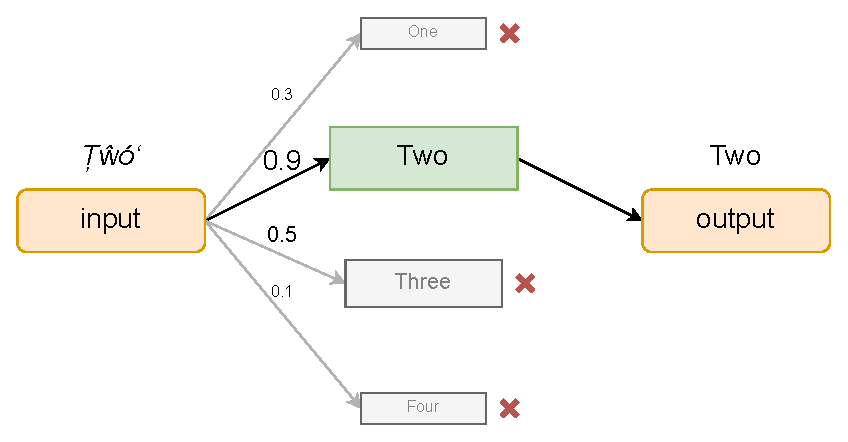
\includegraphics[width=1.0\linewidth]{figures/simplified-cleanup.eps}
	\caption{A simplified representation of a cleanup memory module. The module outputs the SP most similar to the input.}
	\label{fig:simplified-cleanup}
\end{figure}

A convenient consequence of how cleanup memory works is that the output of the cleanup memory can recurrently be fed back into the input. The recurrent connection is scaled by a constant $0 < \alpha < 1$. $\alpha$ needs to be large enough so that the memory keeps its old value but small enough so that a newly provided input can overwrite it. A cleanup memory connected in this way acts like an indefinite error-correcting \emph{memory state} by keeping an input indefinitely once set until another input is provided. A diagram of these memory states can be seen in Figure \ref{fig:cleanup-state}.

\begin{figure}[h]
	\centering
	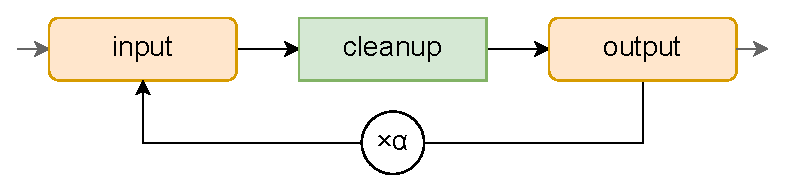
\includegraphics[width=0.9\linewidth]{figures/cleanup-state.eps}
	\caption{An indefinite error-correcting memory state constructed from a cleanup memory with a scaling recurrent connection.}
	\label{fig:cleanup-state}
\end{figure}

\subsection{Managing dynamics}

Another large difficulty when making non-trivial Nengo models is ensuring all operations are given enough time to complete and that they execute in the correct order.

A basal ganglia and thalamus-based action selection mechanism described by \cite{Stewart2010} is the basic building block for sequencing model actions. In this mechanism, each action is associated with a scalar utility. At every timestep, the action with the highest utility is selected and executed.

The most natural way to use this system is by implementing a \emph{state sequence} by keeping the state of the model in an SP and updating it as the algorithm progresses. An example state sequence is shown in Figure \ref{fig:state-sequence}. The ability to follow a state sequence like this is crucial to implementing more complex, multi-step algorithms in Nengo models.

\begin{figure}[h]
	\centering
	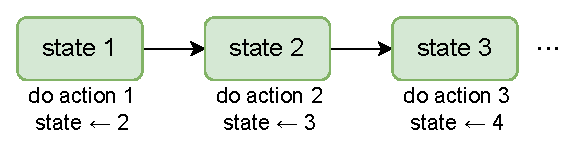
\includegraphics[width=0.7\linewidth]{figures/state-sequence.eps}
	\caption{An example state sequence. At each state, some action is performed, and the next state is set.}
	\label{fig:state-sequence}
\end{figure}

A state-sequence implemented simply as described above has a major flaw. Performing an action and setting a state both happen in parallel. Suppose that performing action 1 takes longer than updating the state from state 1 to state 2. Now the model will progress to state 2 before completing action 1.

Traditionally, this has been solved in models such as the ones by \cite{Aubin2016} and \cite{Praetorius} by splitting up actions over multiple states and by introducing scaling constants into the state transition to control how long updating a state takes. This approach is visualized in Figure \ref{fig:state-sequence-2}.

\begin{figure}[h]
	\centering
	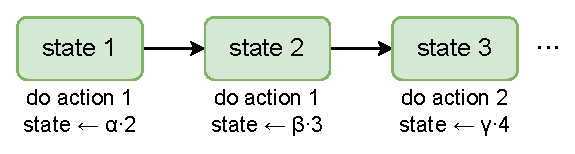
\includegraphics[width=0.7\linewidth]{figures/state-sequence-2.eps}
	\caption{A modified state sequence traditionally used to deal with the model dynamics. Note that action 1 is performed both in state 1 and in state 2, and that every state transition is scaled by a constant.}
	\label{fig:state-sequence-2}
\end{figure}

While this approach certainly does work around the timing issues, it is time-consuming and error-prone. Dozens of scaling hyperparameters are introduced into the model, and each of them must be carefully balanced against each other and the durations of actions. Moreover, once the correct hyperparameters are found, even the slightest change to the model architecture, the number of neurons, learning rates, or other hyperparameters will break the model. If inputs take different amounts of time to process, the model may not work on specific inputs or specific sequences of inputs. This was likely the reason that the model by \cite{Praetorius} only functioned correctly once out of presumably dozens of runs.

Based on how brittle this approach is, it seems unlikely that the brain would work like this. Thus, a more robust approach is more likely. 

The general issue is that both the action and the state update happen simultaneously, even though the state should not progress until the action is fully completed. In an ideal state sequence, these two steps would be decoupled as shown in Figure \ref{fig:ideal-state-sequence}. ACT-R already decouples actions from state updates, and ACT-R models are very robust as a result.

\begin{figure}[h]
	\centering
	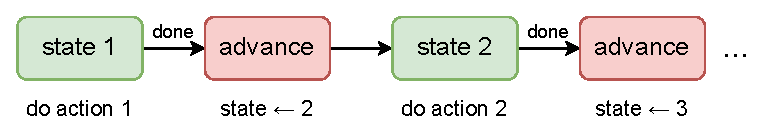
\includegraphics[width=0.9\linewidth]{figures/ideal-state-sequence.eps}
	\caption{An ``ideal" state sequence. The state advances only once the associated action has been completed.}
	\label{fig:ideal-state-sequence}
\end{figure}

Unfortunately, detecting precisely when an action has completed is difficult. One could devise circuits for detecting when specific actions are completed. For example, Figure \ref{fig:done-detector} shows a possible circuit for detecting when a memory state was updated. However, even for such a simple action, the circuit already makes many assumptions about the input. 

\begin{figure}[h]
	\centering
	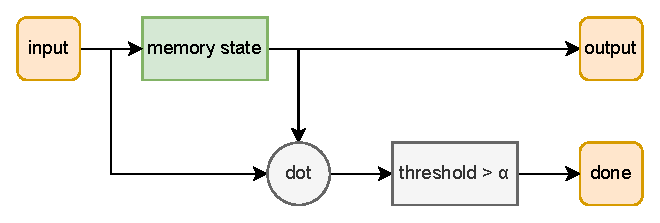
\includegraphics[width=0.9\linewidth]{figures/done-detector.eps}
	\caption{A circuit capable of detecting when the action of setting a memory state has completed. The threshold module outputs 1 when the input is larger than some threshold $\alpha$, and 0 otherwise. The input must be a clean, unit-length SP. Input must only be provided during the action.}
	\label{fig:done-detector}
\end{figure}

It could very well be that building a general circuit for detecting action completeness is not possible. Then each action would require a bespoke circuit. For a complex model with many actions, this may not be feasible. Clearly, a simpler, more scalable solution is needed.

Finally, we turn to computer hardware for a solution. Electrical signals inside a computer chip are generally synchronized via a \emph{clock signal}. This clock is a square wave signal that oscillates at a certain frequency. Each ``action" that a computer performs is designed to take no less than one clock cycle to complete. We applied this idea to circuits built out of spiking neurons instead of electrical ones.

The clock synchronization method was used for all 3 models shown here. The clock was an externally provided square wave. The signal oscillated between \emph{high} (+1) and \emph{low} (-1) on a fixed period. Actions were performed when the clock was high and the state was updated while the clock was low. This is shown in Figure \ref{fig:clock}.

\begin{figure}[h]
	\centering
	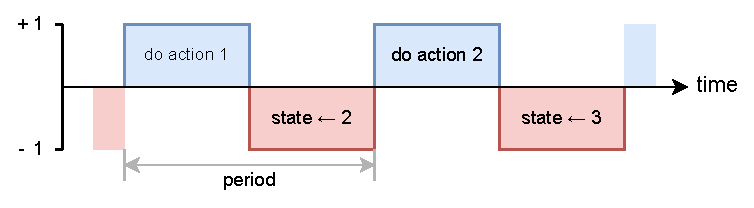
\includegraphics[width=0.9\linewidth]{figures/clock.eps}
	\caption{State sequence synchronized to a clock.}
	\label{fig:clock}
\end{figure}

The clock period is a crucial hyperparameter. It must be tuned such that each action has enough time to complete in one cycle. The clock period can also be tuned further to speed the model up or slow it down in order to match human response times.

\subsection{Counting model}

The counting model was designed to answer a single Zbrodoff problem using only the counting strategy. Algorithm \ref{algo:counting} describes the counting procedure.

\begin{algorithm}[h]
	\begin{algorithmic}
		\State result $\gets$ L
		\State count $\gets$ 0
		\While {count $\neq$ N}
			\State \textbf{increment} result
			\State \textbf{increment} count
		\EndWhile
	\end{algorithmic}
	\caption{Pseudocode for answering letter (L) + number (N) problems using a counting procedure.}
	\label{algo:counting}
\end{algorithm}

Translating the algorithm into the model is relatively straightforward with the help of the previously mentioned memory states and the clock. 

The \emph{result} and the current \emph{count} were both represented by cleanup states. The \emph{increment} operation was implemented using a hetero-associative \emph{incrementing memory}, which mapped each letter or number to its incremented symbol. Two identical incrementing memory modules were used so that the result and the count can both be incremented in parallel. Comparison was performed by a \emph{comparison module} shown in Figure \ref{fig:comparison-module}.

\begin{figure}[h]
	\centering
	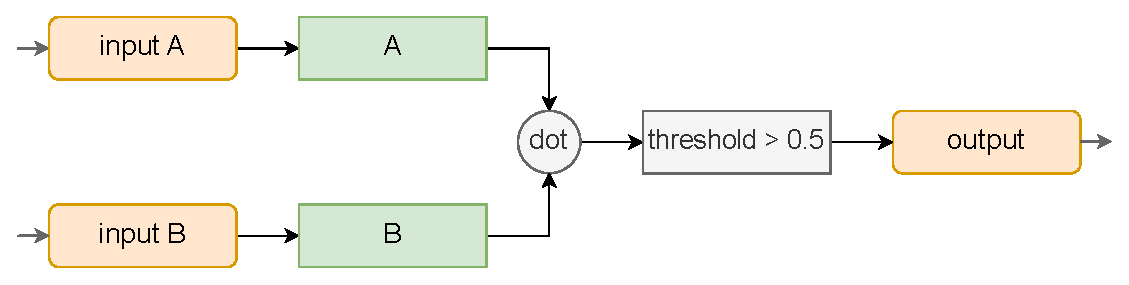
\includegraphics[width=0.9\linewidth]{figures/comparison-module.eps}
	\caption{The comparison module for SPs. Green boxes are memory states from Figure \ref{fig:cleanup-state}. The threshold module outputs +1 when the input is greater than some threshold, and -1 otherwise. The exact threshold value can be any arbitrary value close to 1. 0.5 was used here.}
	\label{fig:comparison-module}
\end{figure}

A flowchart of the model's state sequence can be seen in Figure \ref{fig:counting-model}. The count and letter are incremented preemptively in the Increment state, but the results of the increments are not actually written back until it is determined that counting had not finished. This was done in order to better match human response times.

\begin{figure}[h]
	\centering
	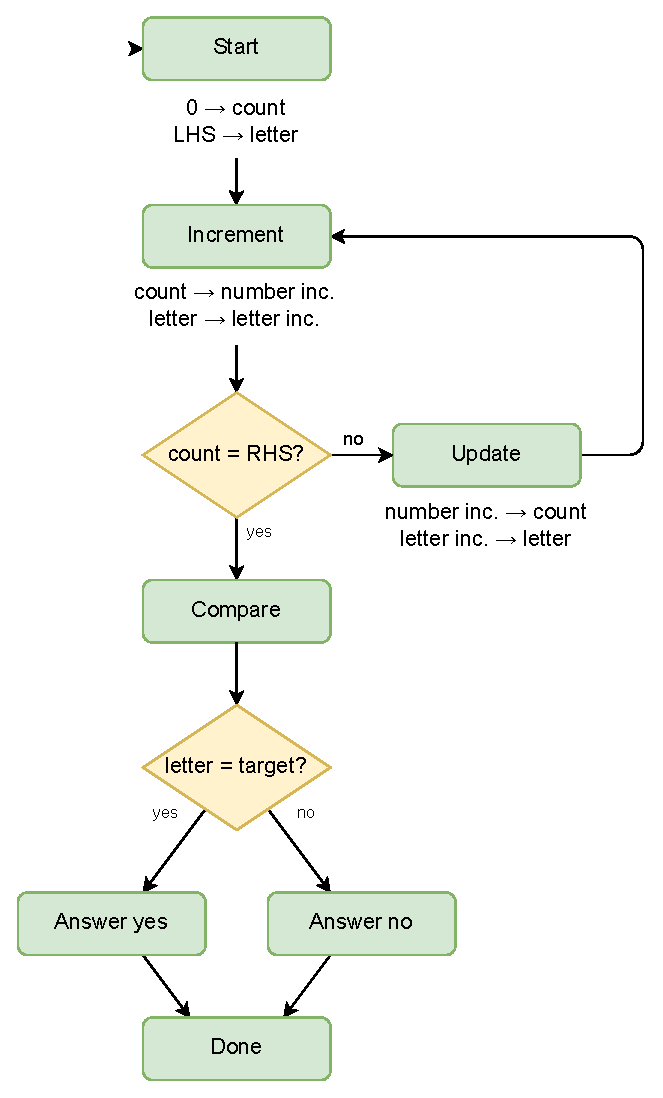
\includegraphics[width=0.8\linewidth]{figures/counting-model.eps}
	\caption{The state flowchart for the counting model. Green nodes represent states. Orange boxes represent decision points. Number increment and letter increment are 2 identical incrementing memories. Letter and count are memory states. LHS represents the left-hand side of the Zbrodoff problem (the letter), while RHS represents the right-hand side (the number).}
	\label{fig:counting-model}
\end{figure}

The counting model consisted of roughly 22\,000 neurons.

\subsection{Learning model}

The learning model was designed to answer a sequence of Zbrodoff problems via only the recall strategy. The model is built around a \emph{declarative memory module}, shown in Figure \ref{fig:declarative-module}.

\begin{figure}[h]
	\centering
	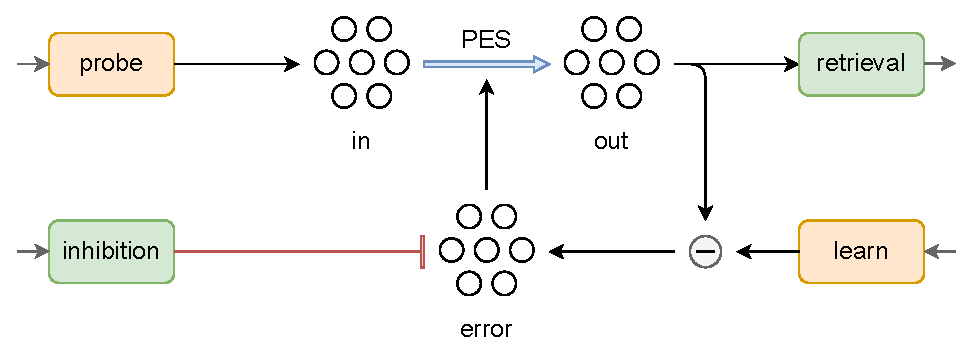
\includegraphics[width=0.9\linewidth]{figures/declarative-module.eps}
	\caption{The declarative memory module used in the learning model and the combined model. Green nodes represent memory states, orange nodes represent simple inputs, dotted arrangements represent simple ensembles. The connection between the in and out ensembles (blue arrow) learns to output the learn signal when probed with a given probe signal. The inhibition state can be used to toggle learning. The red line represents inhibition.}
	\label{fig:declarative-module}
\end{figure}

The declarative module learns associations between an SP presented as $\hat{\text{Letter}} + \hat{\text{Number}}$ and the result using the \emph{prescribed error sensitivity} (PES) learning rule developed by \cite{Arsalidou2011}.

PES adjusts the decoders of every neuron in an ensemble so that the output more closely matches a desired value. The change to a single decoder is calculated according to:

$$\Delta \vec{d}(t) = \kappa a(t) \big(\vec{x}_{desired}(t) - \vec{x}(t)\big)$$

Where $\kappa$ is a learning rate, $a$ is the activation of the neuron, and $\vec{x}_{desired}$ is the desired output.

As can be seen from the equation, once the output error reaches 0, the decoders will no longer be changed, which will stop the learning from taking place. The declarative module also includes an inhibition input, which can be set to manually clear the error to 0 to prevent the model from learning when it is not appropriate. This inhibition was not used in the learning model, but it was used later in the combined model.

PES is a supervised learning rule, so proper examples of input-output pairs need to be provided. Later on, the output of counting can be used for this, but for the learning model, an ideal, pre-defined associative memory was used to feed the error signal.

Typically, a learned associative memory such as this one also uses the unsupervised, \emph{vector Oja} (Voja) learning rule developed by \cite{Voelker2014}. While PES modifies neuron decoders, Voja modifies the encoders and tries to specialize specific neurons to each input.

Input specialization solves the problem of catastrophic forgetting with PES, where adjusting the decoders for one desired output completely overwrites the previously learned decoders for another output. However, Voja has its own version of the forgetting problem, where neurons flip back and forth between encoding two different inputs. This problem can be solved by setting a high intercept value for all neurons in the input ensemble \citep{Knight2016}.

Voja was already successfully used with PES in the model by \cite{Aubin2016}, however, we found that it was unnecessary for our models. Instead, simply setting the intercept to a high value (a hyperparameter) was enough to specialize the neurons to particular inputs.

The learning model consisted of roughly 18\,000 neurons.

\subsection{Combined model}

The combined model is designed to solve a sequence of Zbrodoff problems. Initially, the model uses the counting strategy until it learns the answers. After that, the model uses the recall strategy. Algorithm \ref{algo:counting} describes the combined procedure. This procedure is equivalent to the one used by the ACT-R model.

\begin{algorithm}[h]
	\begin{algorithmic}
		\State result $\gets$ \textbf{recall} L + N = ?
		\If {recall was \emph{not} successful}
			\State result $\gets$ L
			\State count $\gets$ 0
			\While {count $\neq$ N}
				\State \textbf{increment} result
				\State \textbf{increment} count
			\EndWhile
		\EndIf
		\State \textbf{learn} L + N = result
	\end{algorithmic}
	\caption{Pseudocode for answering letter (L) + number (N) problems using a combined counting and recall procedure.}
	\label{algo:combined}
\end{algorithm}

Note that the model is only supposed to count when it could not successfully recall. However, detecting whether a recall succeeded is not a trivial matter. As a result, this functionality was not implemented in the final combined model. Instead, the model always counted for the first 75 seconds of the simulation and then always recalled for the rest of the simulation.

The state sequence of the final model can be seen in Figure \ref{fig:combined-model}.

Since the probe is a combination of two SPs, it was not stored in a memory state. As a result, the model was constantly setting the probe signal, regardless of whether recall was needed in the current state.

\begin{figure}[h]
	\centering
	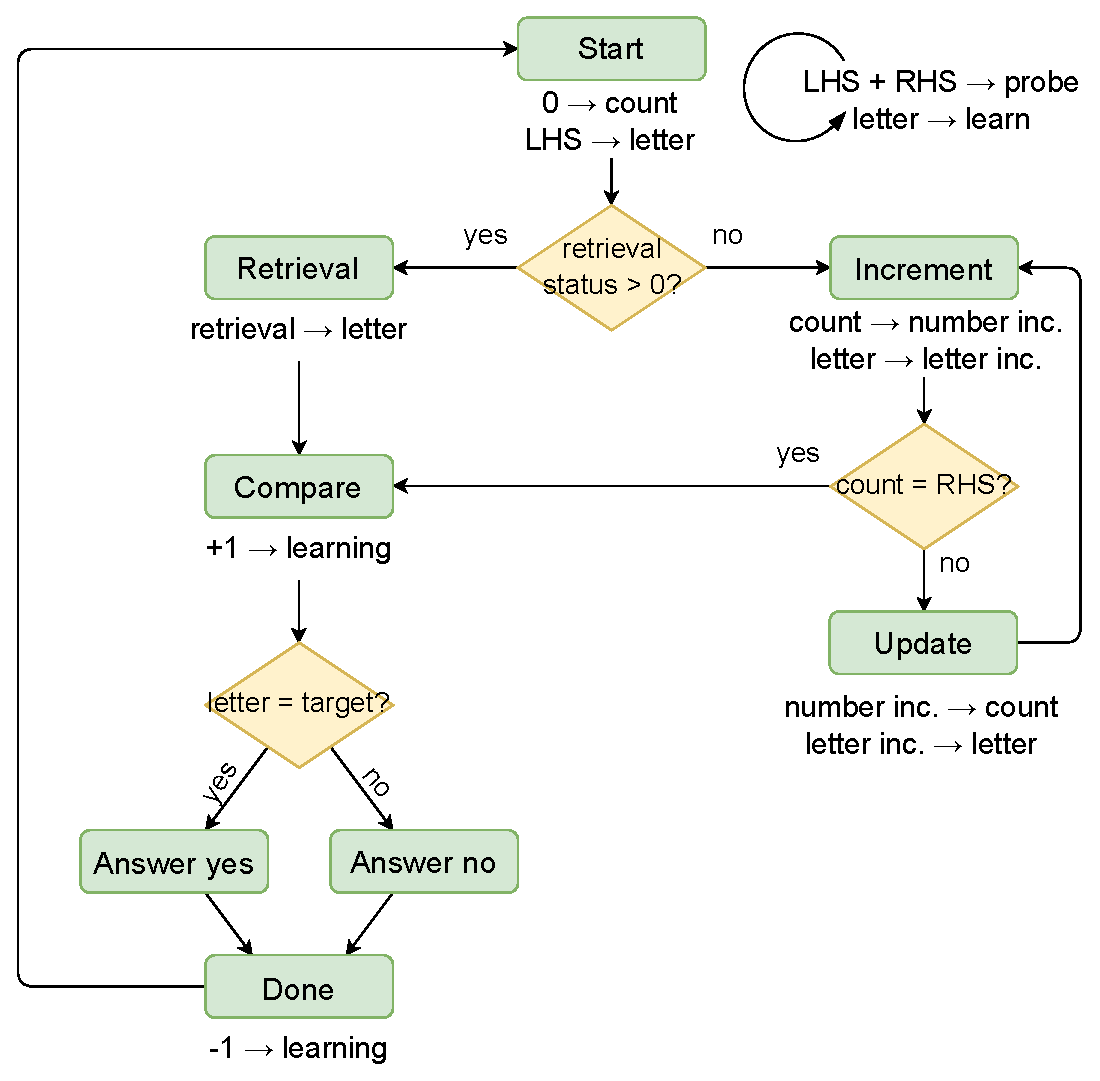
\includegraphics[width=0.95\linewidth]{figures/combined-model.eps}
	\caption{The state flowchart for the combined model. Green nodes represent states. Orange boxes represent decision points. Number increment and letter increment are two identical incrementing memories. Letter and count are memory states. LHS represents the left-hand side of the Zbrodoff problem (the letter), while RHS represents the right-hand side (the number).}
	\label{fig:combined-model}
\end{figure}

For each problem, the model will count if the retrieval status is positive, otherwise, the counting is skipped, and the retrieval results are used instead. Once an answer is obtained from either method, learning is enabled until the model gives an answer.

The combined model consisted of roughly 48\,000 neurons.

\subsection{Hyperparameters}

The hyperparameters used for all 3 models are shown in Table \ref{table:hyperparameters}. They were generally tuned so that the same values worked for each model. They were also tuned with the intent of using as few neurons as possible. The clock period was tuned to match the response times from \cite{Zbrodoff1995} experimental data.

\begin{table}[h]
	\centering
	\begin{tabular}{lccccc}
		model    & $D$ & $N$ & $P$  & $\kappa$ & $I$ \\\hline
		counting & 16  & 64  & 0.25 & /        & /   \\
		learning & 16  & 64  & 0.25 & 0.001    & 0.5 \\
		combined & 32  & 64  & 0.25 & 0.2      & 0.5 \\
	\end{tabular}
	\caption{The hyperparameters used for each model. $D$ is the number of dimensions used to represent SPs. $N$ is the number of neurons used per dimension. $P$ is the clock period in seconds. $\kappa$ is the PES learning rate. $I$ is the intercept used for all neurons in the learning ensemble.}
	\label{table:hyperparameters}
\end{table}

The learning rate was not tuned to match the time it took humans to memorize the answers. Each participant in Zbrodoff's experiment went through 576 problems in total, which would have taken days to simulate, and therefore no attempt was made. The learning rate was simply tuned so that the models would be able to recall answers within a more reasonable time frame.

The combined model used a higher learning rate than the learning model because it was given proportionally less time to learn since the counting circuit took up most of the time.

The only other parameter that differs between models is the number of dimensions used to represent SPs. This parameter greatly influences the number of neurons and thus the computational complexity and memory usage of the model. Therefore, lower values were preferred for the counting and learning models. These models also work with 32 dimensions.

\section{Results}

A trace of the counting model answering A + 3 = D and D + 4 = G can be seen in Figure \ref{fig:counting-model-results-yes} and Figure \ref{fig:counting-model-results-no} respectively.
	
\begin{figure}[h]
	\centering
	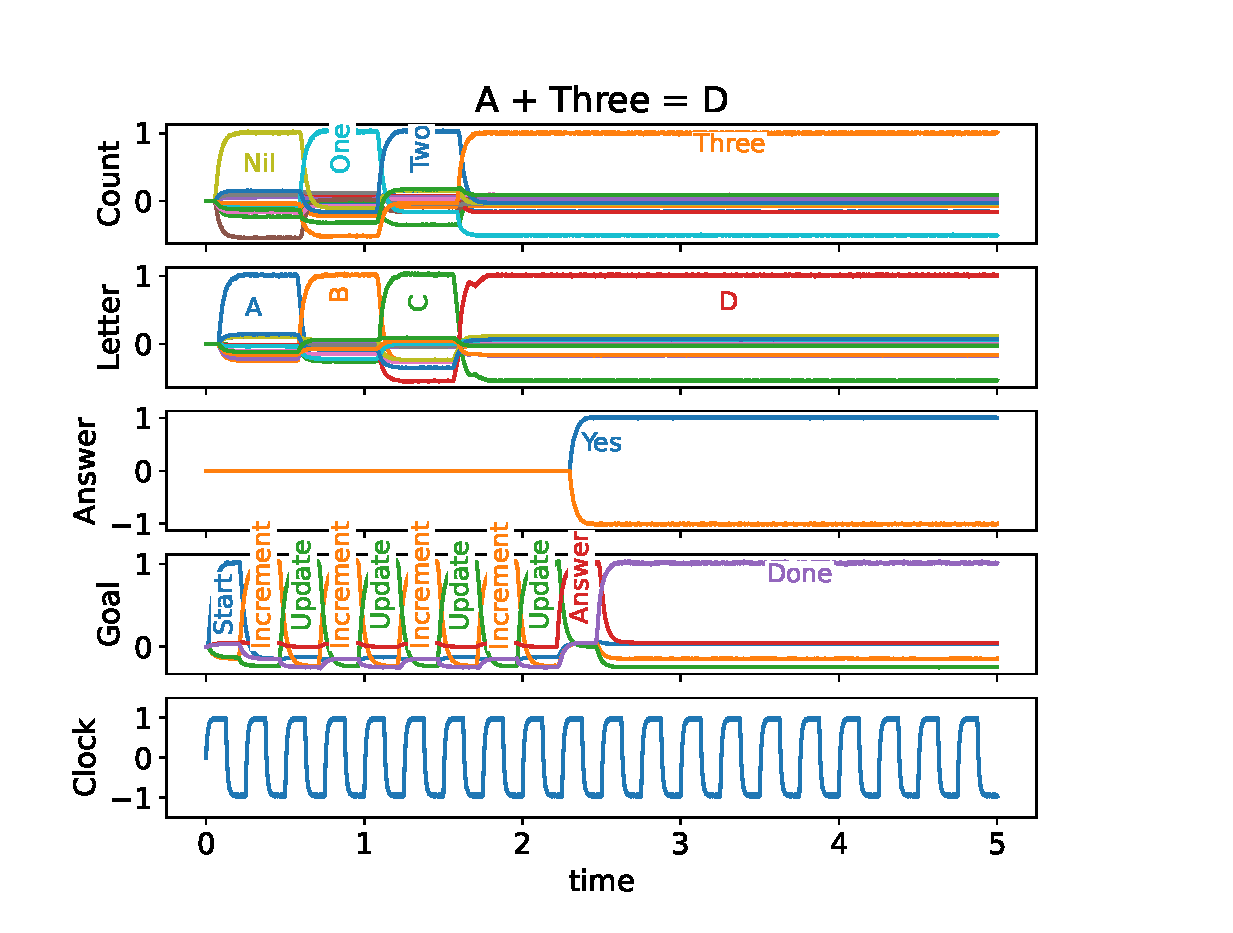
\includegraphics[width=1.1\linewidth]{figures/counting-model-results-yes.eps}
	\caption{A trace of the counting model answering A + 3 = D. Count and Letter represent the working memory of the model. Goal represents the current state.}
	\label{fig:counting-model-results-yes}
\end{figure}

\begin{figure}[h]
	\centering
	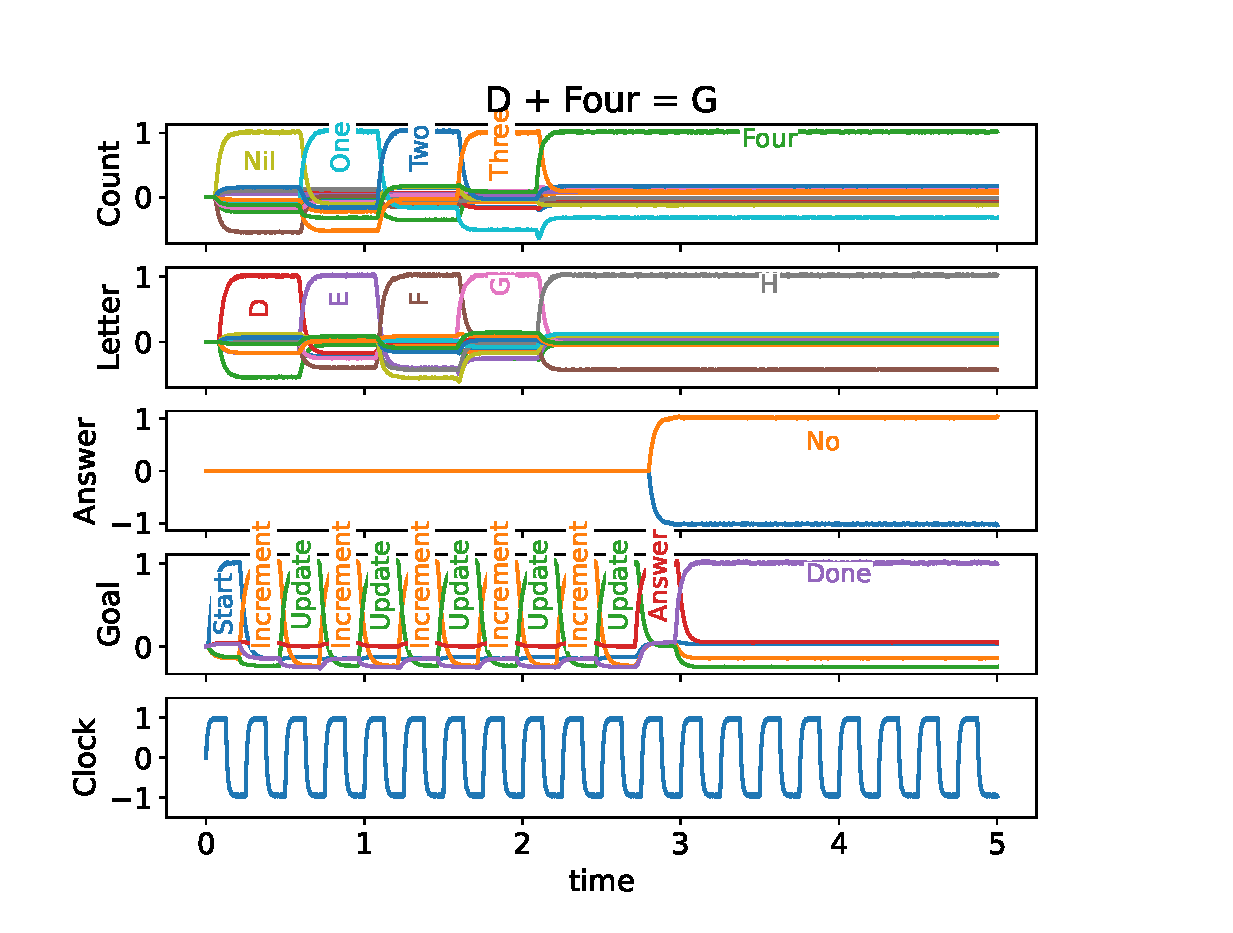
\includegraphics[width=1.1\linewidth]{figures/counting-model-results-no.eps}
	\caption{A trace of the counting model answering D + 4 = G. Count and Letter represent the working memory of the model. Goal represents the current state.}
	\label{fig:counting-model-results-no}
\end{figure}

As shown in the figures, the state transitions occurred cleanly, and the model states contained very little noise. The model was able to count up to the correct result on all 12 possible problems without any issues. The model was also able to give the correct yes/no response to all tested problems.

In order to test the stability and generality of the model, the model was given the problem A + 7 = H, which is outside of the typical range of inputs the model was designed for. The model was not able to answer correctly without modification, but when the SP dimensions were doubled from 16 to 32, the model was able to give the correct answer with no further modifications. A trace of the model answering this problem can be seen in Figure \ref{fig:counting-model-results-stress}.

\begin{figure}[h]
	\centering
	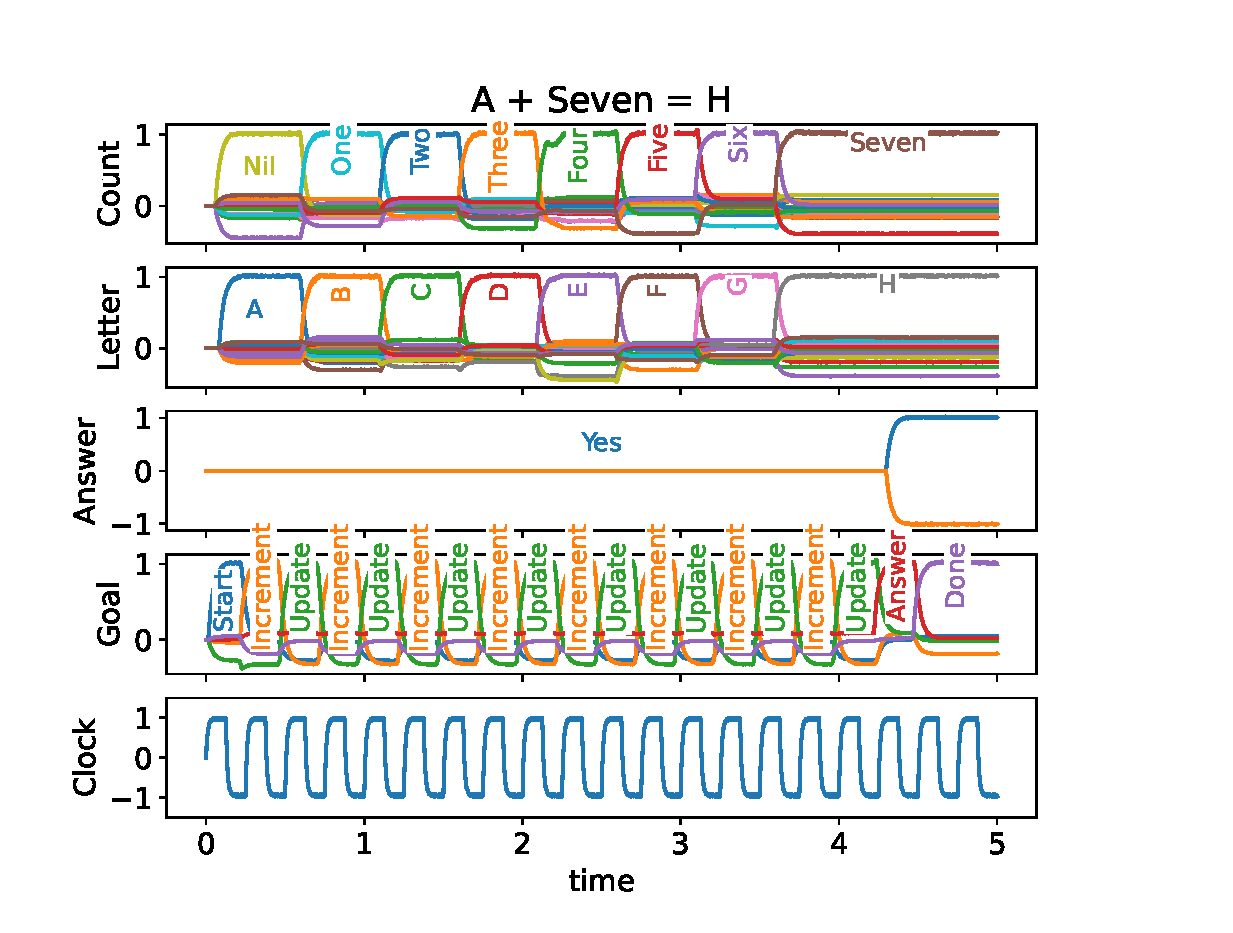
\includegraphics[width=1.1\linewidth]{figures/counting-model-results-stress.eps}
	\caption{A trace of the counting model answering A + 7 = H. Count and Letter represent the working memory of the model. Goal represents the current state. Note that the dimensionality of the SPs needed to be doubled in order to get the correct answer for this problem.}
	\label{fig:counting-model-results-stress}
\end{figure}

The model took 2.555 simulated seconds to respond to A + 3 = D, and it took 3.053 seconds to respond to D + 4 = G. Since the number of steps in the model's algorithm scales linearly with the addend, we can conclude that the model will take approximately 1.05 + 0.5 seconds per addend to respond to a given problem.

The learning model was tested on the following sequence of 6 problems: A+2=C, B+2=D, C+3=F, D+3=F, A+4=D, B+4=G. This sequence contains all 4 possible letters on the left-hand side and all 3 possible addends on the right-hand side, as well as both true and false equations. The inputs were cyclically repeated once the model reached the end of the sequence.

The model ran for 20 simulated seconds, and learning was inhibited after 15 seconds elapsed. The problem sequence was cycled through about 4 times during the simulation. The trace of the model answering these problems can be seen in Figure \ref{fig:learning-model-results}.

\begin{figure}[h]
	\centering
	\includegraphics[width=1.1\linewidth]{figures/learning-model-results.eps}
	\caption{A trace of the learning model answering a repeating sequence of 6 problems. Learning was cut off after 15 seconds when the Inhibition signal dropped to -10. Ideal mem. shows the ideal memory output for the given problem. Retrieval shows the actual output of the declarative module. Note that the model's motor response was not shown here for clarity.}
	\label{fig:learning-model-results}
\end{figure}

As can be seen from the Figure, the retrieval output of the model initially does not match the ideal memory. Over time, the retrieval output and the ideal memory output match more closely. Finally, after approximately 10 seconds (2 full cycles of the problems), the two outputs matched exactly.

The model took approximately 1 second to answer each problem. Furthermore, since the number of steps for each problem is constant for this model, this will be the case regardless of what problem is presented.

Lastly, the combined counting and learning model was tested on a sequence containing all problems A+1=B through D+4=H. This was done in order to somewhat replicate the conditions from the experiment by \cite{Zbrodoff1995}, as well as from the ACT-R model, in which all possible problems were also shown. The problems from the testing sequence were always correct in order to make it easier to verify whether the model was answering correctly.

The model ran for 60 simulated seconds and switched from counting to learning after 45 seconds elapsed. The problem sequence was cycled through about 4 times during the simulation. The trace of the model answering these problems can be seen in Figure \ref{fig:combined-model-results-full}.
	
\begin{figure*}
	\centering
	\includegraphics[width=1.1\linewidth]{figures/combined-model-results-full.eps}
	\caption{A trace of the combined counting and learning model answering a repeating sequence of problems. Learning was cut off after 45 seconds when the Status signal is set to +1.}
	\label{fig:combined-model-results-full}
\end{figure*}

As can be seen in the Figure, the model was able to successfully count during the counting phase, and it was able to memorize the results from the counting for later. The model took around 2 cycles through each problem in order to learn the correct outputs.

When the model was counting, it took on average 2.25, 2.75, and 3.25 seconds to respond to addends 2, 3, and 4, respectively. When the model was recalling, it took 1.25 seconds to respond regardless of the addend. These timings are compared to the human response times from the Zbrodoff experiment, as well the ACT-R Zbrodoff model in Figure \ref{fig:timing-comparison}.

\begin{figure}[h]
	\centering
	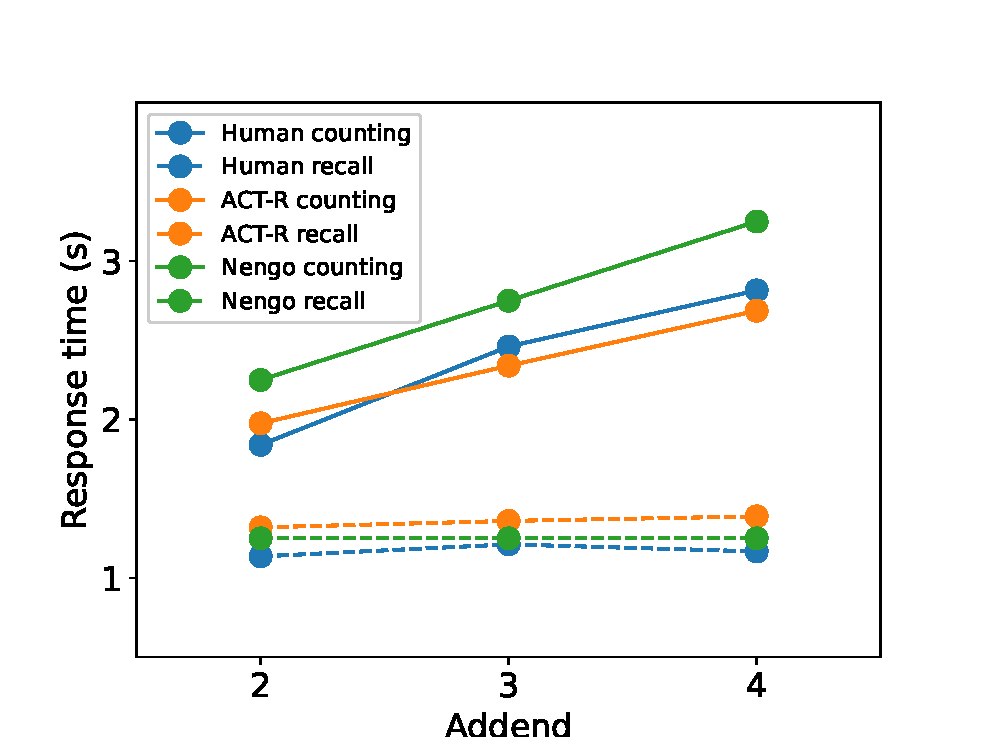
\includegraphics[width=1.0\linewidth]{figures/timing-comparison.eps}
	\caption{A comparison of the response times of the combined counting + learning Nengo model (green), the ACT-R model (orange), and the human experimental data (blue) in block 1 (counting) and block 3 (recall). Solid lines represent the counting strategy response times, while dashed lines represent the recall strategy response times.}
	\label{fig:timing-comparison}
\end{figure}

As can be seen in this comparison, our model generally takes slightly longer to respond than a human. The difference is larger for the counting strategy, where our model takes around 0.5 seconds longer to respond than humans. However, the response times of all 3 models match relatively closely, and they all exhibit similar patterns.
	
\section{Discussion}
	
We set out to develop a cognitive model in spiking neurons capable of performing \citeauthor{Zbrodoff1995}'s alphabet arithmetic tasks, and match human response times, whilst being robust to changes in inputs or hyperparameters.
	
The model presented here is able to solve Zbrodoff problems. It initially uses a counting strategy and slowly memorizes answers. After a fixed point in time, it successfully switches to a recall strategy. The model is robust against changes to hyperparameters and the input, and its results are repeatable, unlike earlier spiking models \citep{Praetorius}. The model also scales to larger problems it was not designed to solve, as was seen in Figure \ref{fig:counting-model-results-stress}. Setting up the model required minimal hyperparameter tweaking, there are only around 10 important hyperparameters, unlike the similar model by \cite{Aubin2016} which had over 40 hyperparameters. Our model uses only 50\,000 neurons, while \citeauthor{Praetorius}' model uses 360\,000.

As could be seen in Figure \ref{fig:timing-comparison}, our model is able to reproduce the general pattern of response times compared to the experimental data from \cite{Zbrodoff1995}. However, it should be noted that the model always responded slightly more slowly than humans. This is a bigger issue than is at first apparent because both humans and the ACT-R model also needed time to visually parse each problem, as well as to respond to each problem, but our model did not spend any time on these tasks.

Unfortunately, some corners were cut in the design of the model. First and foremost, the model has no internal mechanism for detecting when to switch over from counting to recall. This functionality was already implemented in earlier models by \cite{Aubin2016} and \cite{Praetorius}. Also, the model relies heavily on an external clock signal for dynamics control, but there does not seem to be much evidence for the existence of such signals in the brain. We will now discuss potential solutions to these problems.

\subsection{Detecting the success of recall}

Currently, the model decides whether to count or recall based on a retrieval status signal. This signal should, in theory, be high when the model is able to remember a previous answer to the current problem and low when it is not able to remember. However, in the final implementation shown here, this signal is always low for a pre-specified period of time and then high afterward. Several approaches for this problem have already shown promise before.

\cite{Praetorius} seems to have used a simple threshold-based strategy. The declarative module is initially set up to output only 0 vectors for all inputs. As the model learns over time, the magnitude of the retrieved value will increase as it approaches the ideal value (which is unit length). The retrieval status can then be implemented as the squared magnitude of the retrieved vector. 
Unfortunately, this simple approach did not work for our model, at least not consistently. While the model is learning associations, sometimes it would initially learn an association incorrectly. For example, it might learn A + 2 = B, even though it was correctly being taught A + 2 = C from counting. This likely happens when the SPs for B and C are similar, and so the learned vector temporarily passes through the vector for B while heading towards the vector for C. If we had used a higher number of dimensions, then the average similarity between SPs could be smaller, which may fix this issue. However, this would not scale or generalize well as there is always the possibility of two SPs being generated similarly given a large enough vocabulary. On the other hand, participants in the Zbrodoff experiment were not provided any feedback on whether they answered correctly or not. Without this feedback it is entirely possible that some of the participants learned the answers incorrectly in a similar manner to this. So this approach could likely be used to model this behavior.

Alternatively, the approach used by \cite{Aubin2016} is to compare the SP that would have been retrieved with the counting result. Only once the retrieval and counting results are equal for a certain period of time does the model switch from the counting strategy to retrieval. This approach works, however, it is not robust and does not scale. The model does not decide whether to count or retrieve on a per problem basis but rather always counts or always retrieves. If the model is shown a new, unseen problem after it has switched to retrieval mode, it will never learn the new problem. A human would likely be able to recognize that the new problem was never seen before.

Yet another approach was used by \cite{Voelker2014}. Their associative memory module seems to learn an additional value for each key. The module learns the key-value pair like our declarative module, but it also learns a scalar value that goes from 0 to 1. Through learning, this scalar value would eventually settle to 1 around the same time as the actual association was learned, so the scalar could be used as a retrieval status. It is not entirely clear whether this approach would be very robust since it would likely take longer to learn the whole association than to learn a single scalar value.

Perhaps the approaches of \cite{Aubin2016}, and \cite{Voelker2014} could be combined to create a robust method for detecting recall success. Whenever the model finishes counting, the result would be compared to the SP that would have been retrieved for that problem, and the retrieval status for that particular problem would be learned based on the similarity between the outputs of the two approaches.

\subsection{Alternatives to the clock}

The clock signal that was introduced to the model in order to simplify the complex dynamics of spiking neurons turned out to be a potent tool. The clock allowed us to not worry about exactly how the model progresses from one state to another or exactly how long a state needs to last in order for its action to complete. The clock made the model more robust, repeatable, and more understandable than similar models such as the one by \cite{Aubin2016}. 

The clock effectively eliminated the need to manually tune the dynamics of every state transition, which is usually a very time-consuming process. The stability provided by the clock also made it possible to use significantly fewer neurons in the model. This, in turn, reduced the time spent running and testing the model. The development time saved by the clock could then be used to develop other areas of the model, such as the declarative module.

Finally, the clock makes it easy to tune the model's response time to experimental results, at least in principle. In practice, a single clock cycle needs to take at least as long as the longest action, so there is an upper bound on how quickly the model can be made to run. Also, even if one action takes a relatively short amount of time, the clock will make it take as long as the longest action, which is not very efficient. This particular problem can be solved by splitting up longer actions over multiple states. The clock cycle can then be tuned to last as long as the shortest action instead of the longest. This would allow for finer-grained control of the model timings.

As valuable as the clock proved to be in designing our model, there, unfortunately, is not much evidence that brain circuits run on a clock like this. How the brain circuits sequence operations through time is still poorly understood \citep{Finnerty2015}. Even if the brain does use a clock to sequence some operations, how would it tune the clock so that the operations are given the correct amount of time to complete? This is still an open question.

Even if the brain does not use a clock for sequencing actions, some mechanism for determining how long each action should last is still necessary. Without such a mechanism different actions begin overlapping each other leading to incoherent output. ACT-R's production selection mechanism already implements perfect action sequencing, and ACT-R models behave in a well defined manner. However, all actions in ACT-R have clearly defined results and so detecting when one action ends and another should begin is relatively simple. This is not the case in Nengo, where neuronal dynamics are a concern.

Previous models by \cite{Aubin2016} and \cite{Praetorius} used something like a \emph{fuse} mechanism, in which each action was fine-tuned to take a specific amount of time to advance the state to the next action while completing. Unfortunately, this mechanism poses many of the same questions as the clock: how would the brain tune these fuse timings for every action? Also, as we have already discussed, models using this timing method are very fragile. A small change in inputs or hyperparameters completely breaks the control flow. It seems rather unlikely that a computer as error-tolerant as the brain would rely on such a fragile mechanism.

Another possible action sequencing mechanism would simply require that every action be able to measure its own completion. As different actions produce different results, every action would require a dedicated circuit for this task. An example circuit for a simple action was shown in Figure \ref{fig:done-detector}. As can be seen from that Figure, even a very simple action would require complex circuitry to detect its own completion. More complex actions would likely require equally more complex detection circuitry. Given the relative simplicity of the clock or even the fuse mechanisms, a complex solution like this one seems unlikely. On the other hand, this is the only mechanism of the 3 that does not require learning the timings of actions.

The clock, fuse, and completion detection mechanisms all have upsides and downsides, and they each seem implausible in the brain in their own way. Perhaps this suggests some other yet undiscovered mechanism of action sequencing which the brain could easily implement. More research is needed in this area. Until then, the clock mechanism used here has proven very easy to implement and results in more robust, stable, and smaller models than the fuse mechanism that is currently in use.

\subsection{Conclusion}

A robust model of \citeauthor{Zbrodoff1995}'s alphabet arithmetic problems was implemented in spiking neurons. The model initially uses a counting strategy, but it memorizes its previous answers over time and switches to a recall strategy, mimicking a transition from the cognitive learning phase to the associative learning phase.

The transition from counting to recall is manually specified as the model is not able to detect when a previous answer had been completely memorized, however, some suggestions for implementing this behavior were proposed.

The model is built around a clock circuit that is used to synchronize its actions, which made it significantly simpler to develop and reason about while also making it robust against changes in hyperparameters, and generalizable across different inputs. This suggests that the brain works in a similar way, perhaps with a small clock circuit sequencing every action. At the very least, our methodology suggests that \emph{some} mechanism for robustly transitioning between different states is needed. Since current evidence for the existence of a clock in the brain is inconclusive, we discussed an alternative mechanism for sequencing actions through completeness detection.

Memory states composed of cleanup memories were another crucial component needed for action sequencing in our model. They allowed the model to store a clean representation of values which persist across different states and actions. This suggests that similar cleanup states are also present in the brain, particularly in working memory.

Currently, the model is not able to match the human response times from Zbrodoff's experiment, however, it does come close. The model does exhibit similar patterns in response times. Hopefully, it can serve as a groundwork for a future model which is able to completely recreate the timings from the 3 blocks of the Zbrodoff experiment, just like the existing ACT-R models.

\bibliographystyle{plainnat}
\bibliography{references}
	
\end{document}
